\documentclass{beamer}


\usepackage{listings}
\lstset{ % General setup for the package
    language=C,
    numbers=left,
    frame=tb,
    tabsize=4,
    columns=fixed,
    showstringspaces=false,
    showtabs=false,
    keepspaces,
    commentstyle=\color{brown},
    keywordstyle=\color{blue},
    stringstyle=\color{red},
    title=\lstname,
    basicstyle = \tiny,
    breaklines=true,
}

\usecolortheme{beaver}
\setbeamertemplate{navigation symbols}{}
\setbeamertemplate{footline}[frame number]

\title{Street-fighter}
\subtitle{EE-310 Microprogrammed Embedded Systems}
\author[Thür, Mheni]
{Simon~Thür \and Lokman~Mheni}
\institute[EPFL]{EPFL SEL-BA5}
\subject{Microprogrammed Embedded Systems}

\begin{document}
\frame{
    \titlepage
}
\frame{
    \frametitle{NDS features: checklist}
    \framesubtitle{Part 1 of 3}
    \begin{itemize}
        \item ARM Processors
              \begin{itemize}
                  \item ARM9: Screens, Arrow keys, and permanent storage
                  \item ARM7: Wifi and Sound
              \end{itemize}
        \item Timers / Interrupts
              \begin{itemize}
                  \item Used for Countdown (Timer and Interrupt)
                  \item Used for Attack delay (Timer and Interrupt)
              \end{itemize}
        \item Graphics
              \begin{itemize}
                  \item Main screen TODO MODE with TODO BACKGROUNDS ACTIVE
                  \item Sub screen TODO MODE with TODO BACKGROUNDS ACTIVE
              \end{itemize}

    \end{itemize}}

\frame{
    \frametitle{NDS features: checklist}
    \framesubtitle{Part 2 of 3}
    \begin{itemize}
        \item Keypad (polling)
              \begin{itemize}
                  \item \texttt{KEY\_LEFT/KEY\_RIGHT} move player
                  \item \texttt{KEY\_X} jump
                  \item \texttt{KEY\_A} Normal Attack
                  \item \texttt{KEY\_B} Special Attack
                  \item \texttt{KEY\_Y} Block
              \end{itemize}
        \item Touchscreen
              \begin{itemize}
                  \item Select game mode
                  \item Start new round
              \end{itemize}
        \item Sound
              \begin{itemize}
                  \item Play music module in loop when game begins
                  \item Play soundeffects when jumping and attacking
              \end{itemize}
    \end{itemize}
}


\begin{frame}
    \frametitle{NDS features: checklist}
    \framesubtitle{Part 3 of 3}

    \begin{itemize}
        \item Secondary storage
              \begin{itemize}
                  \item Storing most rounds won
                  \item Reading most rounds won
              \end{itemize}
        \item Wifi
              \begin{itemize}
                  \item Send and receive Player position
                  \item Send and receive Damage done
                  \item Send and receive game control / sync instructions
              \end{itemize}
        \item Sprites
              \begin{itemize}
                  \item Use sprites to display local and remote characters
              \end{itemize}

    \end{itemize}

\end{frame}


\begin{frame}
    \frametitle{NDS project screenshot}
    \begin{figure}
        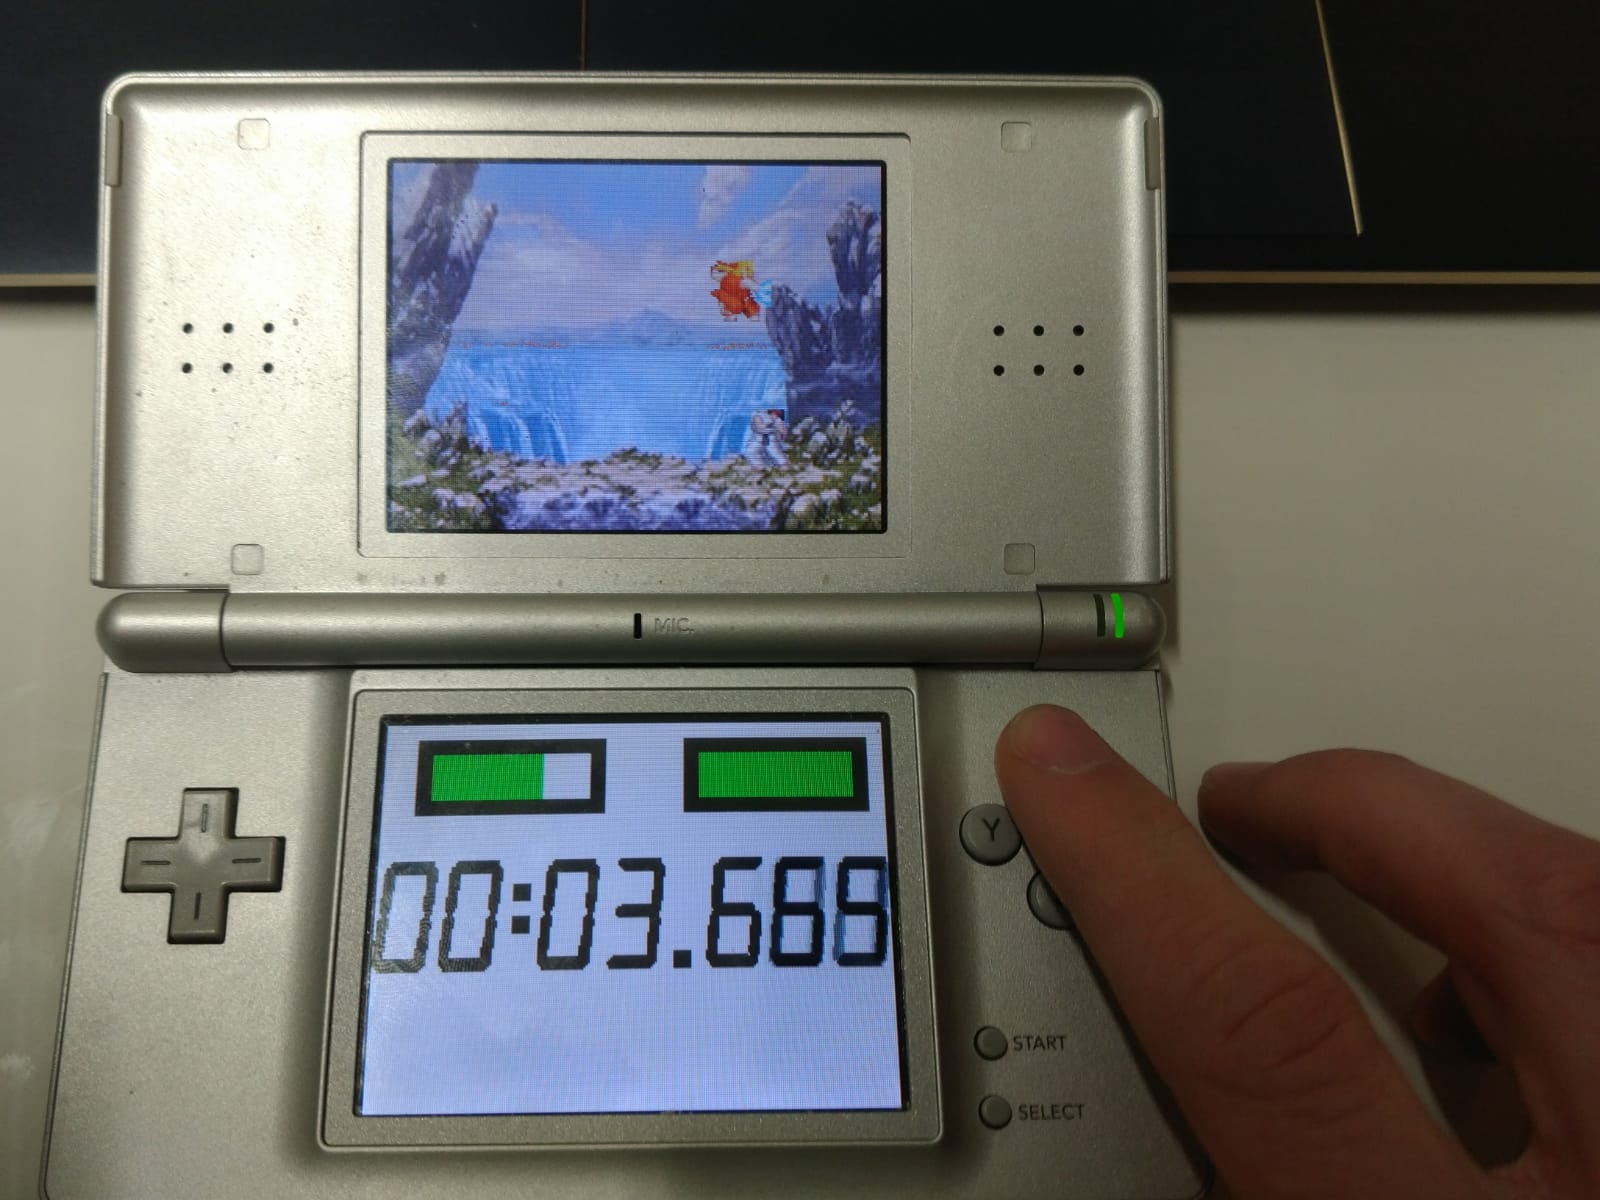
\includegraphics[width=\textwidth]{imgs/example.jpeg}
    \end{figure}
\end{frame}


\end{document}